\section{Results}\label{sec:results}

\subsection{Model Building}

We build models as described in \secref{sec:training}. A few different model
types are shown in \figref{fig:models}.

\begin{figure*}
  \centering
  \begin{subfigure}[]{0.3\linewidth}
    \centering
    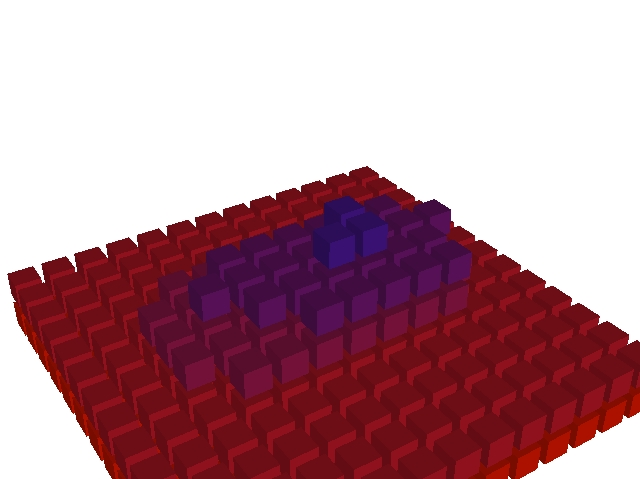
\includegraphics[height=1.5in]{figures/car_marginal.jpg}
    \caption{Na\"ive Bayes}
    \label{fig:nb}
  \end{subfigure}
  \begin{subfigure}[]{0.3\linewidth}
    \centering
    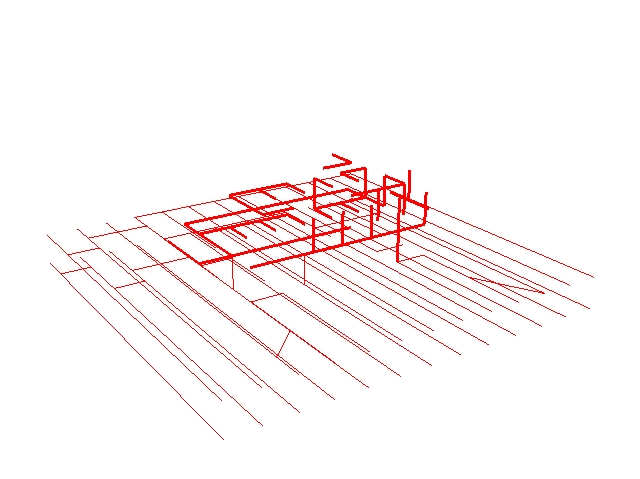
\includegraphics[height=1.5in]{figures/car_tree.jpg}
    %\caption{An example of a \ac{CLT} built for a car. For easier viewing, edges
    %  in the tree that link to nodes that are usually unoccupied are not rendered,
    %  and edges above the ground plane are rendered as thicker lines.}
    \caption{\ac{CLT}}
    \label{fig:clt}
  \end{subfigure}
  \begin{subfigure}[]{0.3\linewidth}
    \centering
    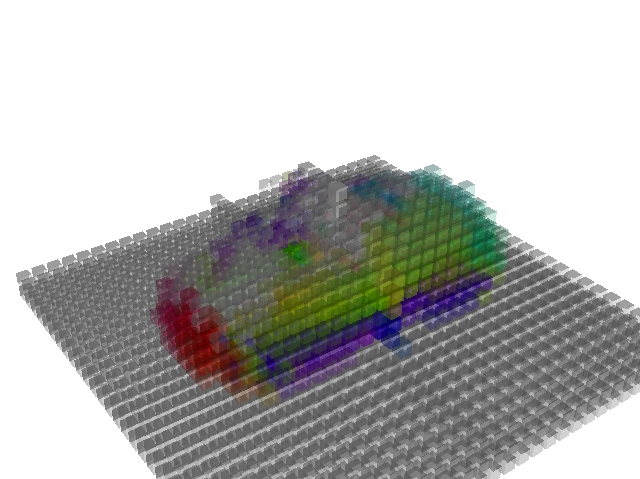
\includegraphics[height=1.5in]{figures/car_fm.jpg}
    \caption{Surface Normals}
    \label{fig:sn}
    %\caption{An example of a model with surface normals. Each voxel is colored by
    %  the most commonly observed surface normal orientation. The hue represents the
    %  surface normal's rotation about the vertical axis, and the saturation
    %  represents the surface normal's angle from the xy plane.}
  \end{subfigure}
  \caption{In \figref{fig:nb}, we see an example of a Na\"ive Bayes model for a
    car. Voxels are colored by z-height, and only voxels that are likely to be
    occupied are rendered. In \figref{fig:clt}, we see the \ac{CLT} as computed
    over the model. Only edges between voxels that are usually occupied are
    shown, with edges above the ground plane rendered as thicker lines. In
    \figref{fig:sn}, we see the model augmented with surface normals. Each voxel
    is colored by the most commonly observed surface normal orientation. The hue
    represents the surface normal's rotation about the vertical axis, and the
    saturation represents the surface normal's angle from the xy plane.}
  \label{fig:models}
\end{figure*}

\subsection{Detection Results on KITTI Object Challenge}

While demonstrating some promising results, \ldots

\begin{itemize}
  \item 1-gram (independence assumption)
  \item Greedy Approximation
  \item Full \ac{CLT}
\end{itemize}

\subsection{Runtime Performance}

On average, it takes \aku{\unit{1 million}{\sec}} to process \aku{...}
